%\documentclass[handout]{beamer}
\documentclass{beamer}
\usepackage[utf8]{inputenc}
\usepackage[T1]{fontenc}
\usepackage[official]{eurosym}
\usepackage[english,swedish]{babel}
\usepackage{booktabs}
\usepackage[iso,swedish]{isodate}
\usepackage{acro}
\usepackage{tabularx}
\usepackage{url}
\usepackage{varioref,prettyref}
\usepackage{graphicx}
\usepackage{color}
\usepackage{subfig}
\usepackage[style=alphabetic,maxbibnames=99,backend=biber]{biblatex}
\setbeamertemplate{bibliography item}[text]
\usepackage[varioref,prettyref]{miunmisc}

\addbibresource{msbintro.bib}

\mode<presentation>{
  \usetheme{Boadilla}
  \usecolortheme{}
  \usefonttheme{professionalfonts}
  \setbeamercovered{transparent}
}

\setbeamerfont{frametitle}{size=\footnotesize}
\setbeamerfont{framesubtitle}{size=\tiny}

\DeclareAcronym{isms}{
  short = ISMS,
  long = Information Security Management Systems,
}

\title[Intro infosäk]{%
  Introduction to\\
  Swedish Civil Contingencies Agency (MSB) methodological support for introducing \ac{isms}.
}
\author{Lennart Franked\footnote{Based on material written by
    Carina Bengtsson and Daniel Bosk}}
\institute[MIUN IST]{%
  Department of Informationsystem and Technologies (IST),\\
  Mid Sweden University, Sundsvall.

  %Avdelningen för informations- och kommunikationssytem (IKS),\\
  %Mittuniversitetet, Sundsvall.
}

\date{\today}

\pgfdeclareimage[height=0.65cm]{university-logo}{MU_logotyp_int_CMYK.pdf}
\logo{\pgfuseimage{university-logo}}

\AtBeginSection[]{%
	\begin{frame}<beamer>{Overview}
		\tableofcontents[currentsection]
	\end{frame}
}
\AtBeginSubsection[]{%
	\begin{frame}<beamer>{Overview}
		\tableofcontents[currentsection, currentsubsection]
	\end{frame}
}
\AtBeginSubsubsection[]{%
	\begin{frame}<beamer>{Overview}
    \begin{center}
      \insertsubsubsectionhead{}
    \end{center}
	\end{frame}
}
\begin{document}

\begin{frame}
  \titlepage{}
\end{frame}

\begin{frame}{Overview}
	\tableofcontents
	% You might wish to add the option [pausesections]
\end{frame}

\section[Information Security]{Information Security}
\subsection{Introduction to Information Security}

\begin{frame}{Why do we as a society need this?}
  \begin{itemize}
    \item Information is central in today's society.
    \item Accommodates the need for both the individual and the society.
    \item Necessary to avoid disturbances in our information systems.
  \end{itemize}
\end{frame}

\begin{frame}{Tieto incident}
  \begin{itemize}
    \item In 2011 Tieto got a hardware problem in one of their
      datacenters~\cite{Lindkvist2012tdf}. This created disruptions in many of
      the companies customers IT-system. For example: 
      \begin{itemize}
        \item All the pharmacies got problems handing out prescription medicin for a
          time.
        \item The swedish vehivle inspection agency could not report the results
          from the vehicle inspections they did during this time.
        \item A large logistical company could not handle its operation
        \item Social offices in Nacka and Sollentuna were unable to pay child
          support
      \end{itemize}
  \end{itemize}
\end{frame}
\begin{frame}{1177 incident}
  \begin{itemize}
    \item In 2019 a sub-contractor of a sub-contractor for a company that was
      handling the IT-system for three swedish regions health care guides (1177)
      call line, forgot to secure a backup server that stored the recordings
      from the phone calls~\cite{Ottsjo2019}.
    \item Resulted in around 2.7 million (around 170 000 hours) of recordings of
      confidential phone calls got accessible for the public.
    \item The recordings contains everything from medical symptoms to social
      security numbers.
  \end{itemize}
\end{frame}
\begin{frame}{The Swedish Transport Agency}
  \begin{itemize}
    \item In 2017 it was revealed that sensitive information from the Swedish
      Transport Agency database were made available for non-security screened
      employees abroad~\cite{SvTTransport2017}. 
    \item Information included:
      \begin{itemize}
        \item Driver licences (including picture)
        \item Company secrets
        \item Sensitive information about infrastructure (bridges, subways etc)
        \item Information that can be used to identify armoured cars.
      \end{itemize}
  \end{itemize}
\end{frame}

\begin{frame}{Swedish Public Employment Service}
  \begin{itemize}
    \item In 2019 it was found that the Swedish Publich Employment Services
      (arbetsförmedlingen) automatic system for reporting activity reports to
      the Swedish Social Insurance Agency (Försäkringskassan) sent incorrect
      reports~\cite{SvTPublicEmpl2019}.
    \item It was estimated that 10 to 15 percent of the decisions were incorrect.
    \item Resulted in that approximately 70 000 decisions could have been wrong.
  \end{itemize}
\end{frame}

\begin{frame}{What is information security?}
  \begin{itemize}
    \item Occurs together with other processes and organisations.
    \item Information security in an organisation does not have a value by
      itself. It needs to be integrated into the organisation to be effective.
  \end{itemize}
\end{frame}

\begin{frame}{What is information security?}
  \begin{itemize}
    \item Ability to preserve the requirements and expectations that exist on
      information in an organisation.
    \item Amongst other to protect towards disruptions, such as the previously
      mentioned examples.
  \end{itemize}
\end{frame}

\begin{frame}{Demands and expectations on information}
  \begin{description}
    \item[Confidentiality] The information should only be accessible to an
      authorized entity.

    \item[Availability] The information must be accessible when it is needed.

    \item[Integrity] The information is exact and complete.

  \end{description}
\end{frame}

\begin{frame}{Demands and expectations on information}
  \begin{description}
    \item[Traceability] Who have taken part of, or changed the information?
    \item[Non Repudiation] It should not be possible to deny an act.
    \item[Authentication] Establish an entities identity.
    \item[Authorization] To give an authenticated entity certain permissions.
  \end{description}
\end{frame}

\begin{frame}{What is information security?}
  \begin{figure}
    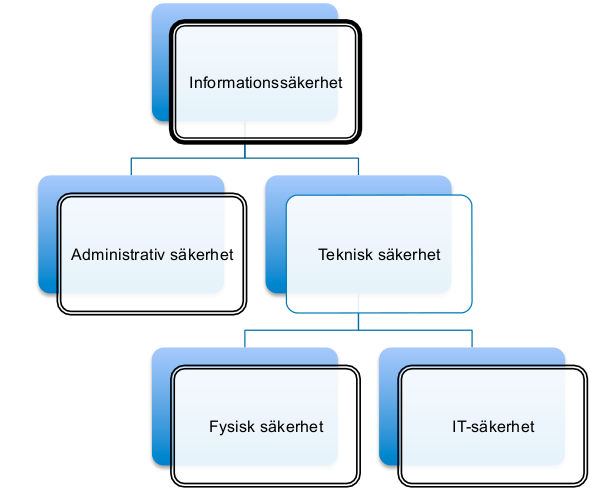
\includegraphics[height=0.7\textheight]{Figures/infosak-struktur.png}
    \caption{Structure of information security.}
  \end{figure}
\end{frame}

\begin{frame}{Structure}
  \begin{figure}
    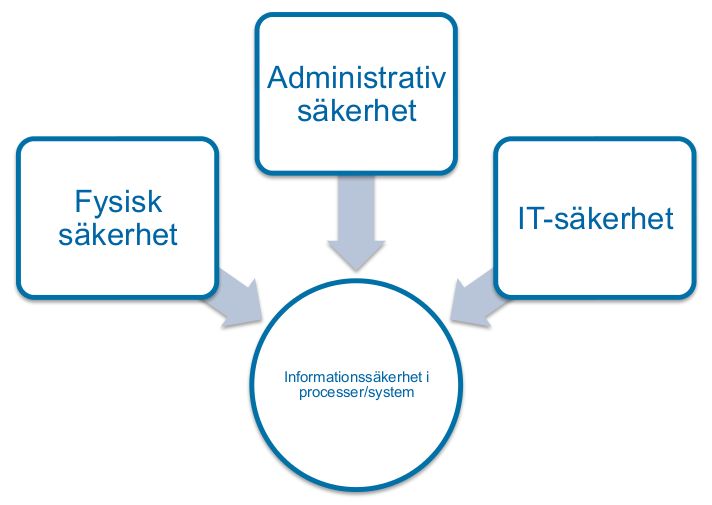
\includegraphics[height=0.7\textheight]{Figures/infosak-process.png}
    \caption{To work with information security}
  \end{figure}
\end{frame}

\begin{frame}{The security isn't stronger than the weakest link}
  \begin{itemize}
    \item Strong password, written down on a post-it next to where it should be
      used.
    \item High grade lock on a regular glass door.
    \item The conditions must be there, in order to be able to work safely.
  \end{itemize}
\end{frame}

\begin{frame}{Why protect the information?}{Non-mandatory}
  \enquote{Good for business}
  \begin{description}
    \item[Reputation:] Who will let a company handle their information, if the
      company is known for treating their data carelessly.
    \item[Financial:] Strong reputation is better for the economy, and the cost
      of dealing with security incidents will be less.
    \item[Internal efficiency:] No loss of information or disruptions in the
      work.
    \item[Quality:] This will hopefully lead to a increase in work quality.
  \end{description}
\end{frame}

\subsection{Information Security Management System}
\begin{frame}{Management System}
  \begin{itemize}
    \item Everyone have a \enquote{system} to manage an organisation.
  \end{itemize}
      A formalized system that is used to make the work more efficient in
      regards to set goals. It should include routines and delegation of
      responsibilities for how the organisation should be managed. It must exist
      clear goals and guidelines for how they should be achieved.
  \begin{itemize}
    \item Covers amongst other, organisational structures, governance documents
      etc.
  \end{itemize}
\end{frame}

\begin{frame}{Information Security Management System (ISMS)}
  \begin{itemize}
    \item Should be integrated with the other management systems!
    \item Refers to how to regulate the work with information security.
    \item Also how to regulate work routines, methods \dots
    \item Governance documents have an important role to play in \ac{isms}\@.
  \end{itemize}
\end{frame}

\begin{frame}{Apply \ac{isms}}
  Not only establish, but also
  \begin{itemize}
    \item implement,
    \item pursue,
    \item monitor,
    \item audit,
    \item maintain and improve
  \end{itemize}
\end{frame}

\begin{frame}{Governance documents}
  \begin{itemize}
    \item Plan of action, policies, guidelines, \dots
    \item Policy: What do we want to achieve?
      One extensive, or multiple smaller ones.
    \item The governance documents should be integrated into the organisations
      current structure.
  \end{itemize}
\end{frame}

\begin{frame}{Committed management}
  \begin{itemize}
    \item How to succeed?
      Support is needed from the top management.

    \item Since the work with information security should cover the entire
      organisation, it is vital that the top management is fully committed.

    \item Those that have been appointed to work with information security,
      needs to have the mandate to be able to do their work.

  \end{itemize}
\end{frame}

\begin{frame}{Create commitment}
  \begin{itemize}
    \item The top management have the overall responsibility for the
      organisation --- This involves information security and security incidents.
    \item Important to make the management understand the importance of
      information security.
  \end{itemize}
\end{frame}

\begin{frame}{Motivation}
  \begin{itemize}
    \item What positive effects might come with strong information security?
    \item What is the price of \emph{not} protecting the information?
      \begin{itemize}
        \item Leaked company secrets.
        \item Inaccessible infrastructure.
      \end{itemize}
    \item Show incidents.
    \item Laws and other regulations?
  \end{itemize}
\end{frame}

\subsection{ISO 27000}
\begin{frame}{ISO 27001}
  \begin{itemize}
    \item ISO 27001 is a continuous process that strives towards constant
      improvements on how to work and use different security solutions in
      regards to information security.
    \item It is important to adapt this after the organisation, but this doesn't
      mean that parts can be skipped.
  \end{itemize}
\end{frame}

\begin{frame}{ISO 27002 --- What should be done?}
  \begin{itemize}
    \item Security Policy.
    \item Organising the information security.
    \item Managing assets.
    \item Human resource and security.
    \item Physical and environmental security.
    \item Control communication and management.
    \item Access control.
    \item Acquisition, development and maintenance of information systems.
    \item Managing information security incidents.
    \item Continuity planning for the organisations.
    \item Compliance.
  \end{itemize}
\end{frame}

\section[Methodilogical support]{MSB:s methodological support}
\begin{frame}{Introduction}{\insertsectionhead}
  \begin{itemize}
    \item Swedish Civil Contingencies Agency (MSB).
    \item \enquote{MSB is responsible for issues concerning civil protection,
        public safety, emergency management and civil defence, as long as no
        other authority has responsibility~\cite[About MSB]{msbse}\@.
        }
    \item This includes protection of our information systems.
  \end{itemize}
\end{frame}

\begin{frame}{Introduction}{\insertsectionhead}
  \begin{itemize}
    \item Support for how to conduct work within information security in an
      organisation.

    \item Explains how to build an information security management system.

    \item Should be seen as a \enquote{smorgasbord}:
      \begin{itemize}
        \item Pick the parts that are related to the organisation.
        \item Apply them in an order that is suitable.
      \end{itemize}

    \item Information security is a complex field:
      \begin{itemize}
        \item It is required that it is integrated in the \emph{entire}
          organisation: From the top management to the lowest operative level.
      \end{itemize}

  \end{itemize}
\end{frame}

\begin{frame}{Overview}{\insertsectionhead}
  \begin{figure}
    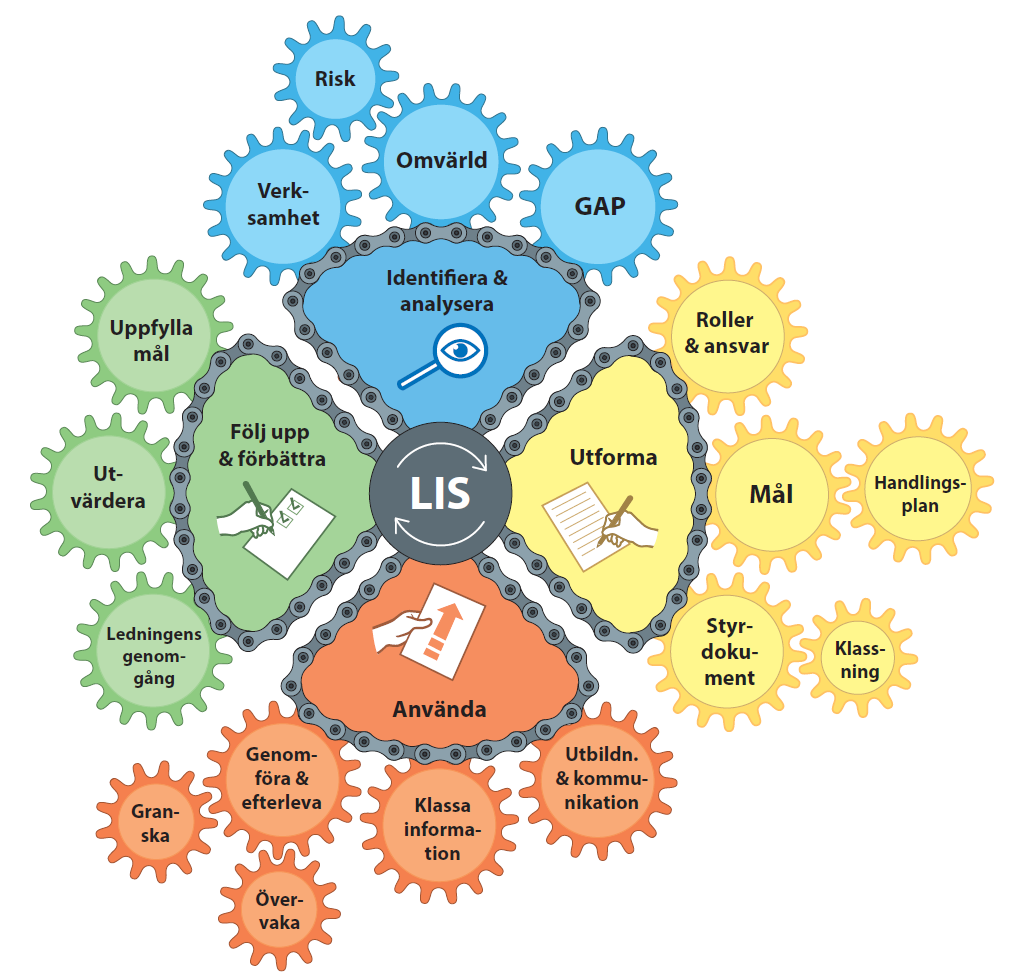
\includegraphics[width=6cm]{Figures/kugghjulet_lis.png}
    \caption{Overview over the methodological support~\cite{msb_metodstod}.}
  \end{figure}
\end{frame}

\begin{frame}{Components}{\insertsectionhead}
  \begin{figure}
    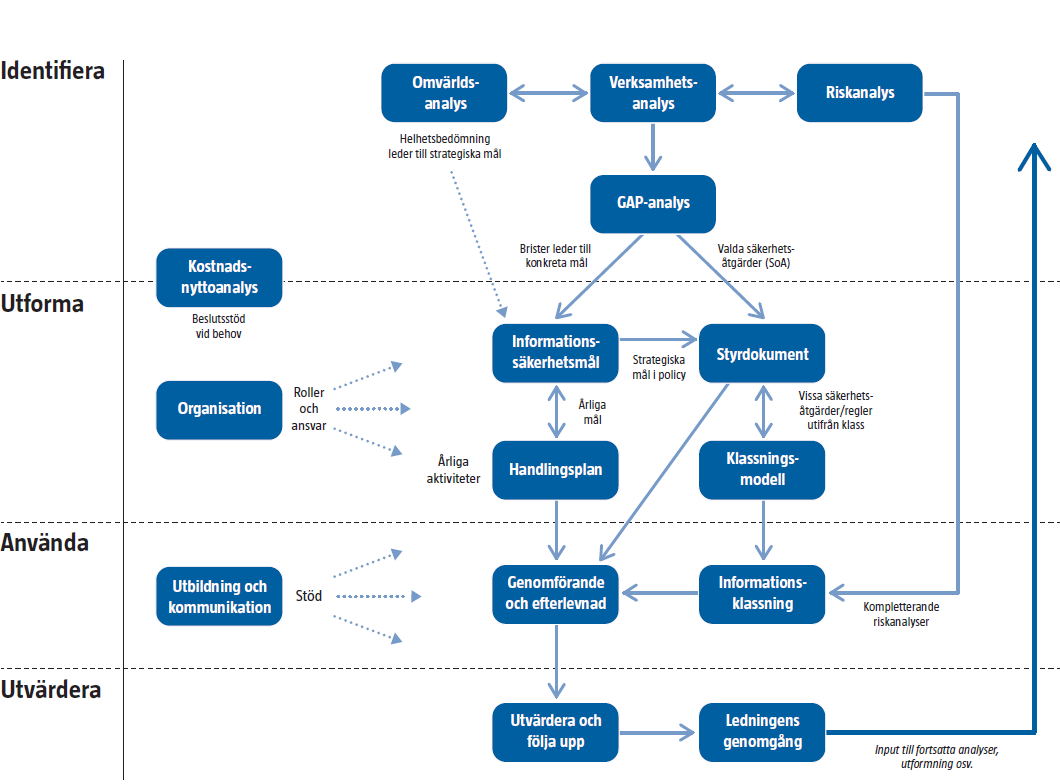
\includegraphics[width=8cm]{Figures/oversiktsbild-over-metodstegens-olika-delar-och-hur-de-relaterar-till-varandra.png}
    \caption{Different parts of the Methodological support~\cite{msb_metodstod}}
  \end{figure}
\end{frame}

\begin{frame}{ISO 27000}{\insertsectionhead}
  \begin{itemize}
    \item ISO 27000 is an international standard covering working with
      information security.
    \item This is not just for governmental agencies.
    \item Any organisation can certify themselves for ISO 27000
    \item MSB:s methodological support is adapted to the international
      standards.
  \end{itemize}
\end{frame}

\subsection{Identify and Analyse}
\begin{frame}{Overview}{\insertsubsectionhead}
  \begin{itemize}
    \item Analyse the external contexts~\footnote{Omvärldsanalys} and the organisation.
    \item Requires knowledge about how the current situation looks
      like~\footnote{Nulägesanalys}.
      \begin{itemize}
        \item Look over existing documentation.
        \item Discuss within the organisation.
      \end{itemize}
    \item Mapping of the informational assets\footnote{informationskartläggning}.
    \item Analyse the risks connected to the informational assets.
    \item Find suitable security measurements.
    \item Existing security measurements are controlled using a GAP-analysis
  \end{itemize}
\end{frame}

\subsubsection{Analysing External and Legal Requirements (Omvärldsanalys)}
\begin{frame}{Analyse External Requirements}{\insertsubsectionhead}
  \begin{itemize}
    \item Mapping 
      \begin{itemize}
        \item External parties needs and expectations
          \begin{itemize}
            \item Customers
            \item Suppliers
            \item Citizens
            \item Reviewers
          \end{itemize}
        \item Prerequisites
          \begin{itemize}
            \item Technical
            \item Social
            \item Environmental
            \item Political
          \end{itemize}
      \end{itemize}
  \end{itemize}
\end{frame}
\begin{frame}{Example of external parties}
  \begin{table}
    \footnotesize
    \caption{Example of external parties~\cite{msb_metodstod}}
    \begin{tabularx}{\textwidth}{X X X}
      Category & Party & Requirement, Role or\newline Impact\\
      \toprule
      Suppliers: &
      \begin{itemize}
        \item Suppliers
        \item Sub-suppliers
        \item Outsourcing partners
        \item In sourcing partners
        \item Cloud Service Providers
        \item Business Partners
        \item Security Providers
      \end{itemize} &
      An organisation is dependent on suppliers, can for example require \newline
      how the supplier is working with information security.\\
    \end{tabularx}
  \end{table}
\end{frame}

\begin{frame}{Legal Requirements}
  \footnotesize
  \begin{description}
    \item[General Data Protection Regulation (GDPR)] Managing personal data.

    \item[Public Access to Information and Secrecy Act 2009:40] Says that
      certain information \emph{must} be available for the public, while other
      information should \emph{not} be.

    \item[The Archives Act 1990:782] Controls what documents that the
      authorities should preserve, that they should be ordered and looked after.
			It also controls how the documents can be disposed. Documents can not be
			disposed if that hinders the right to be able to provide access to official
			documents, research purposes or legal proceedings.
    \item[MSBFS 2016:1] Regulations regarding how governmental agencies should
      work with information security.
  \end{description}
  \begin{block}{Remember!}
    When going through the legal requirements, it is beneficial to get judicial
    expertise.
  \end{block}
\end{frame}
\begin{frame}{MSBFS 2016:1}
  \begin{itemize}
    \item Due to increased electronic information exchange in the society, there
      is now demands put on how governmental agency work with information
      security.
    \item The code of statutes came into effect \printdate{2010-02-01}.
  \end{itemize}
\end{frame}

\begin{frame}{GDPR}{General Data Protection Regulation}
  \begin{itemize}
    \item Replacing Personal Data Act 1998:204
    \item Regulates how personal data are allowed to be stored and used.
      \begin{itemize}
        \item Protects a persons right of privacy~\cite[art. 5]{eu:gdpr}
        \item Personal data can only be stored for as long as there is a need
          for it~\cite[art. 5]{eu:gdpr}.
        \item Each person must give explicit consent to a company/organisation
          to store, publish or share personal data about them~\cite[art.
          7]{eu:gdpr}.  
        \item Ensure that a person have the right to get access
          to all personal
          data that has been collected about them~\cite[art. 15]{eu:gdpr}.
        \item Persons right to erasure~\cite[art. 17]{eu:gdpr}. 
      \end{itemize}
  \end{itemize}
\end{frame}
\begin{frame}{GDPR cont.}{General Data Protection Regulation}
    \begin{itemize}
      \item Possibility to transfer personal data (data
          portability)~\cite[art. 20]{eu:gdpr}.  
      \item Data protection by design and default~\cite[art. 25]{eu:gdpr}.
      \item Records regarding processing activities must be maintained~\cite[art.
        30]{eu:gdpr}.
      \item Personal data breaches must be reported to the supervisory
        authority, without undue delay, not later than 72 hours~\cite[art.
        33]{eu:gdpr}.
    \end{itemize}
\end{frame}
\begin{frame}{GDPR cont.}{General Data Protection Regulation}
\begin{itemize}
    \item Individuals needs to be informed about the personal data
        breach~\cite[art. 34]{eu:gdpr}.
    \item An independent agency should ensure that these rules are 
      followed~\cite[art 51]{eu:gdpr}.
    \item If the organisation does not comply to these regulations, they can be
      fined up to 4\% worldwide turnover or \euro{}20 Million, whichever is 
      greater~\cite[art 83]{eu:gdpr}.
    \item and much more.
\end{itemize}
\end{frame}

\begin{frame}{MSBFS 2016:1}
  1 §  Denna författning innehåller föreskrifter som ansluter till
  bestämmelserna om statliga myndigheters informationssäkerhet i 19§
  förordningen (2015:1052) om krisberedskap och bevakningsansvariga
  myndigheters åtgärder vid höjd beredskap. 
\end{frame}

\begin{frame}{MSBFS 2016:1}
  \footnotesize
  5 §  Varje myndighet ska bedriva ett systematiskt och riskbaserat
  informationssäkerhetsarbete med stöd av ett ledningssystem för
  informationssäkerhet. I detta arbete ska standarderna ISO/IEC 27001:2014 och
  ISO/IEC 27002:2014 beaktas. Tillräckliga resurser ska tilldelas för
  informationssäkerhetsarbetet samt löpande och regelbunden information lämnas
  till myndighetsledningen.

  Detta innebär bland annat att en myndighet måste:
  \begin{enumerate}
    \item upprätta en informationssäkerhetspolicy och andra styrande dokument
      som behövs för myndighetens informationssäkerhet,
    \item utse en eller flera personer som leder och samordnar arbetet med
      informationssäkerhet,
    \item klassificera sin information med utgångspunkt i krav på
      konfidentialitet, riktighet och tillgänglighet,
    \item utifrån risk- och sårbarhetsanalyser och inträffade incidenter
      avgöra hur risker ska hanteras, samt besl uta om åtgärder för
      myndighetens informationssäkerhet,
    \item dokumentera granskningar och säkerhetsåtgärder av större betydelse
      som har vidtagits.
  \end{enumerate}
\end{frame}

\begin{frame}{MSBFS 2016:1}
  10 § Myndigheten ska ha rutiner för att identifiera, rapportera, bedöma,
  hantera och dokumentera incidenter som kan påverka säkerheten i den
  informationshantering som myndigheten ansvarar för eller i tjänster som
  myndigheten tillhandahåller åt en annan organisation. Myndigheten ska ha
  rutiner för att lära av sådana inträffade incidenter och utförda åtgärder.
\end{frame}

\subsubsection{Organisational Analysis\footnote{Verksamhetsanalys}}
\begin{frame}{\insertsubsubsectionhead}
  \begin{itemize}
    \item Mapping
    \begin{itemize}
      \item Internal parties needs, requirements and expectations.
      \begin{itemize}
        \item Decision makers
        \item Object owners
        \item Co-workers
        \item Support units
      \end{itemize}
      \item Internal Prerequisites.
      \begin{itemize}
        \item Goals
        \item Strategies
        \item Organisational Culture
        \item Infrastructure
      \end{itemize}
      \item The organisations essential informational assets.
    \end{itemize}
  \end{itemize}
\end{frame}

\begin{frame}{Analyse Informational Assets}{\insertsubsubsectionhead}
  \begin{block}{Informational Assets}
    Informational assets are the organisations information and its resources
    that deals with information. For example to receive, store, process, show or
    communicate it~\cite{msb_metodstod}.
  \end{block}
\end{frame}

\begin{frame}{Dividing informational assets}{\insertsubsubsectionhead}
  \begin{description}
    \item[Primary] Refers to the main information, such as blue prints, logs or
      contracts.
    \item[Secondary] Refers to resources that are required to access the primary
      informational assets.
  \end{description}
  What will happen if you do not have your program that is required to read the
  closed proprietary format that the information is stored with?
\end{frame}
\begin{frame}{Critical Informational Assets}
  \centering
  \begin{block}{What is a critical informational asset?}
    There are alot of informational assets in an organisation. It is therefore
    necessary to establish what should be considered a critical asset.
  \end{block}
\end{frame}

\begin{frame}{Performing the organisational analysis}{\insertsubsubsectionhead}
  \begin{block}{General analysis}
    Important to only perform a general analysis of the organisation.
  \end{block}
  \begin{block}{Previous Work?}
    Are there any previous analysis available?
  \end{block}
\end{frame}

\begin{frame}{Documenting the informational assets}
  When documenting the informational assets, ensure that at least the following
  is documented:
  \begin{itemize}
    \item Name
    \item Description
    \item Type of information, for example personal data.
    \item Critical?
    \item Owner and contact information
  \end{itemize}
\end{frame}

\subsubsection{Risk analysis}
\begin{frame}{Overview}{\insertsubsubsectionhead}
  \begin{itemize}
    \item Identifies the information security risks.
    \item Can be performed over generally over the organisation, or on a
      specific object.
    \item The identified risks are then assessed based on probability and
      consequence.
  \end{itemize}
  \begin{block}{What to acheive with a risk analysis}
    \begin{itemize}
      \item What can happen?
      \item How probable is it?
      \item What is the consequences?
    \end{itemize}
    Note that the result of the risk analysis shouldn't be seen as the absolute
    truth.
  \end{block}
\end{frame}

\begin{frame}{When should the Risk Analysis be performed?}{\insertsubsubsectionhead}
  \begin{itemize}
    \item Not necessary to perform the risk analysis after analysing the
      organisation or external and legal requirements.
    \item If it is performed after, then the results from these can be used in
      the risk analysis.
    \item Otherwise, it is possible to rely on the existing knowledge of the
      organisation.
  \end{itemize}
\end{frame}
\begin{frame}{When should the Risk Analysis be performed?}{\insertsubsubsectionhead}
  Examples of when it can be suitable to perform a risk analysis.
  \begin{itemize}
    \item Procuring new services?
    \item Outsouring
    \item Organisational changes
  \end{itemize}
\end{frame}

\begin{frame}{How should the process for Risk Analysis look like?}{\insertsubsubsectionhead}
  \footnotesize
  \begin{block}{Already have a process?}
    If the organisation already have a process in place, then this can be used.
    Since it's already well established in the organisation.
  \end{block} 
  \begin{block}{If there isn't a process in place?}
    Some key points to think about when establishing a process for Risk
    Analysis.
    \begin{itemize}
      \item How should the process look like?
      \item What criteria for consequence and probability estimation should be
        used?
      \item What criteria for risk acceptance should be used?
      \end{itemize}
  \end{block}
  \begin{block}{Establish Criterias for Consequence and Probability}
    In IS0 27001:2018 the management are responsible for making a decision
    about the process, criteria for consequence and probability levels, and
    what risk levels should be considered acceptable. 
  \end{block}
\end{frame}
\begin{frame}{Establishing a table for grading consequence}{\insertsubsubsectionhead}
  Create a table for help establishing consequence level connected to each risk.
  For example:
  \begin{itemize}
    \item Financial loss
    \item Negative effect
    \item Infringement
    \item Environmental
    \item Personal Safety
  \end{itemize}
\end{frame}
\begin{frame}{Establishing a table for grading consequence}{\insertsubsubsectionhead}
  \begin{table}
    \tiny
    \caption{Table for helping estimate risk~\cite{msb_metodstod}}
    \begin{tabularx}{\textwidth}{X | X | X | X}
    Consequence & Financial loss & Loss of reputation & Disruption in the
    organisation\\ 
    \toprule

    Severe & Two million SEK and above, or 20\% over budget & Continous negative
    reporting in media or by organised groups in social media. Focused on not
    just individuals but the organisation as a whole.& Disruptions in one or
    several critical organisations that are longer than acceptable.\\

    \midrule
    Considerable & 500 000 - 2 million SEK or 10-20\% over budget & Negative
    reporting in local and national media and in organised social media groups.
    Focused mainly on special instances or actions from a certain individual~(s)
    & Disruption in one critical organisation that are longer than acceptable.
    \\ 
    \midrule
    Moderate & 1 - 500 000 or 5-10 \% over budget & A few dissatisfied
    individuals that express themselves in social medias or a smaller notice in
    local media.& Disruptions in one or several non-critical organisations that
    are longer than acceptable.\\ 
    \midrule
    Negligible & No loss & Little or non negative attention in media or social
    media & Negligable disruption in the organisation\\ 
    \bottomrule
  \end{tabularx}
  \end{table}
\end{frame}

\subsubsection{GAP Analysis}
\begin{frame}{Overview}{\insertsubsubsectionhead}
  \begin{itemize}
    \item Identifies the gap between the current state of the organisation and
      what level of security the organisation wants to achieve.
    \item For example, the current state versus the actions mentioned in ISO
      27001~\cite[Bilaga A]{iso27001}
    \item Develop an action plan on how to fix the objects that aren't 
      sufficient.
  \end{itemize}
\end{frame}

\begin{frame}{Statement of Applicability}{\insertsubsubsectionhead}
  Statement of Applicability (Uttalande om tillämplighet)
  \begin{itemize}
    \item What should be covered in the GAP-analysis?
    \item Select security meassures, either from previous analyses, or pick all.  
    \item Once finished, the organisation have a complete list of security
      meassures that are applicable to the organisation.
  \end{itemize}
\end{frame}
\begin{frame}{Perform the GAP analysis}{\insertsubsubsectionhead}
  Based on the list of applicable security meassures
  \begin{itemize}
    \item Is the security meassure already in place?
    \item Estimate the severity of the security meassure.
    \item Describe the current status of this security meassurement.
  \end{itemize}
\end{frame}
\subsubsection{The Results of the Analysis}
\begin{frame}{The result of the analysis}{\insertsubsubsectionhead}
  \begin{itemize}
    \item The result will act as a base when modelling the information security.
    \item Helps to assess how the organisation handles the information security.
    \item Identifying security measures.
  \end{itemize}
  
\end{frame}

\subsection{Utforma}
\subsubsection{Classifying Information}
\begin{frame}{Classifying information}
  \begin{itemize}
    \item Method to evaluate how much an informational asset is worth
      protecting.

    \item To be able to create a suitable protection.

    \item Evaluate each asset based on:
      \begin{itemize}
        \item Availability,
        \item Integrity,
        \item Confidentiality.
      \end{itemize}

    \item Each perspective have a number of security levels.

  \end{itemize}
\end{frame}

\begin{frame}{MSB:s suggestion on a classification model}
  \begin{figure}
    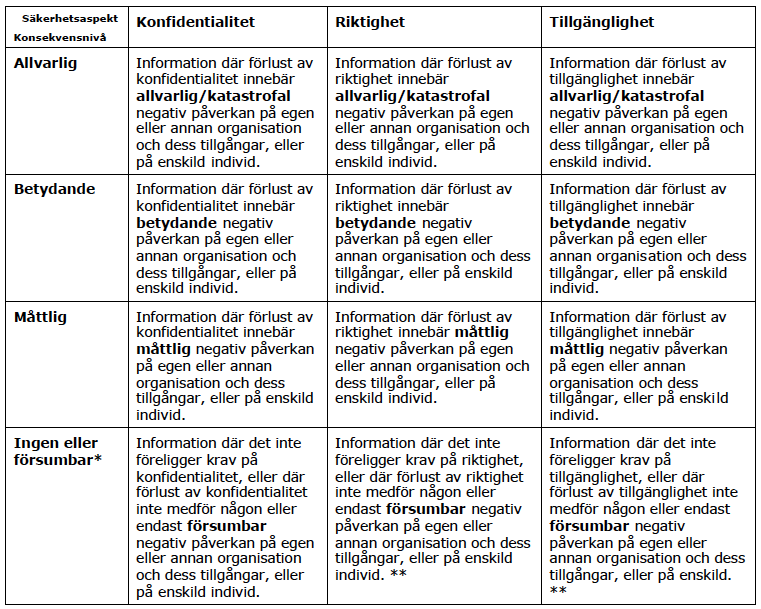
\includegraphics[height=0.7\textheight]{Figures/msb-klassificering.png}
    \caption{MSB:s suggestion on a classification model with levels: Severe, Considerable,
      Moderate, Negligible.}
  \end{figure}
\end{frame}

\begin{frame}{Classifying information}
  \begin{itemize}
    \item All assets are classified using all the identified requirements based
      on all the different perspectives.
    \item The information owner should be the one classifying the information.
    \item It is good to adapt the model based on the organisation.
  \end{itemize}
\end{frame}

\begin{frame}{University's adaptation of a classification model.}
  \begin{figure}
    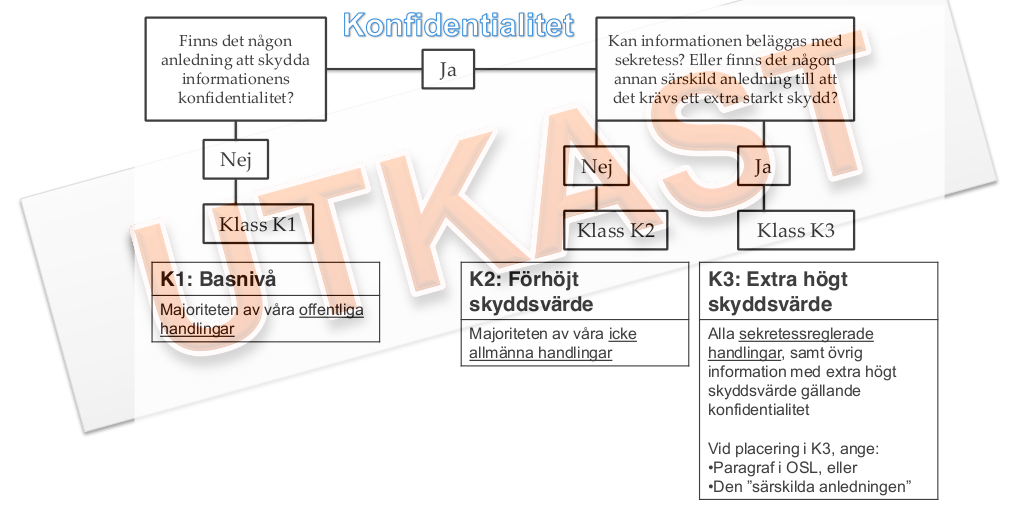
\includegraphics[width=\textwidth]{Figures/miun-klassificering.png}
    \caption{University's adaptation of a classification model from the
      confidentiality perspective.}
  \end{figure}
\end{frame}

\begin{frame}{University's adaptation of a classification model}
  \begin{figure}
    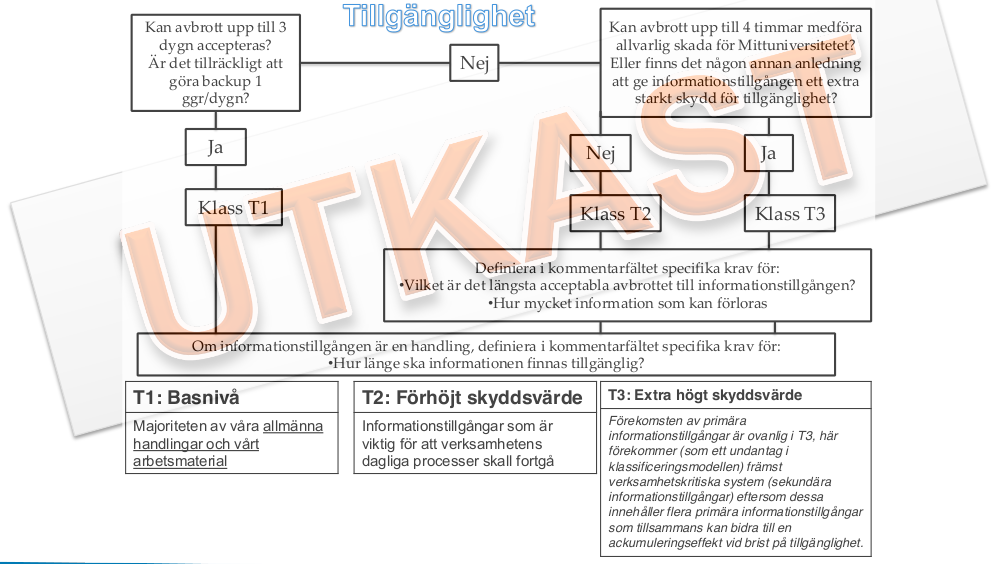
\includegraphics[width=\textwidth]{Figures/miun-tillganglighet.png}
    \caption{University's adaptation of a classification model from the
      availability perspective.}
  \end{figure}
\end{frame}

\begin{frame}{University's adaptation of a classification model}
  \begin{figure}
    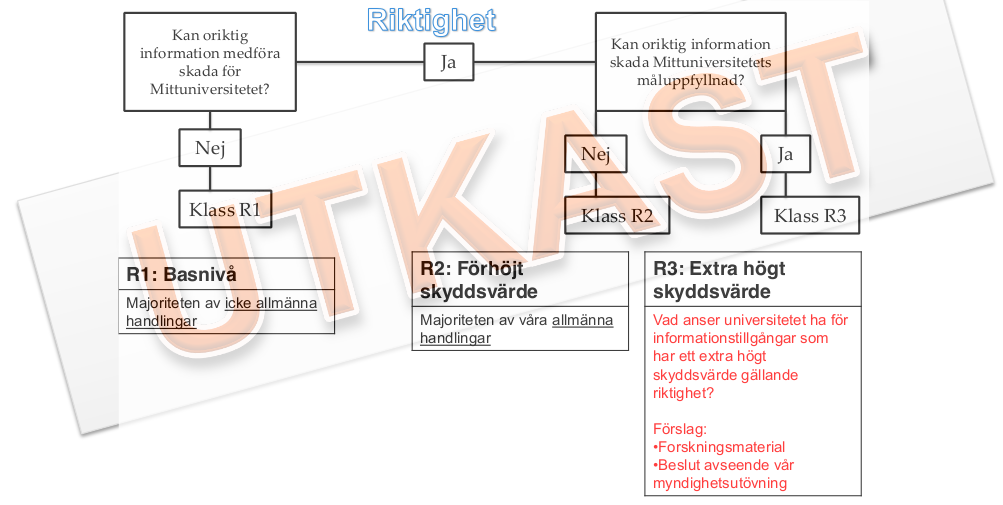
\includegraphics[width=\textwidth]{Figures/miun-riktighet.png}
    \caption{University's adaptation of a classification model from the
      integrity perspective.}
  \end{figure}
\end{frame}

\begin{frame}{Example of the result from the university}
  \begin{figure}
    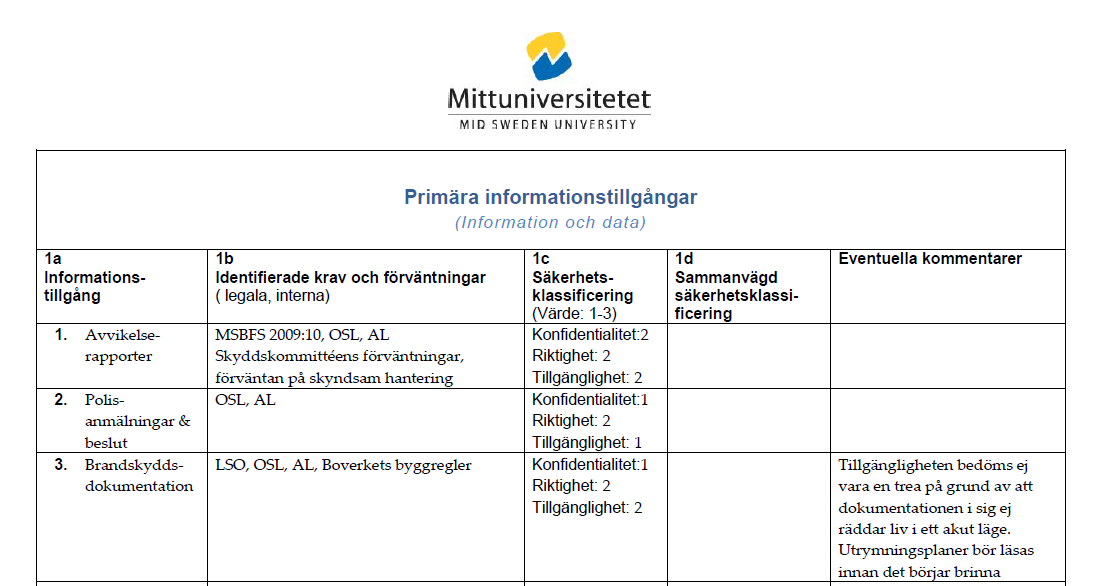
\includegraphics[width=\textwidth]{Figures/miun-klassresultat.png}
    \caption{Part of the result from the university.}
  \end{figure}
\end{frame}

%=======================================================================%



\begin{frame}[allowframebreaks]{References}
	\small
  \printbibliography{}
\end{frame}

\end{document}

